% -------------------------------------------------------------------------------- %

\begin{exercise}[Exercise 4.1]

In Example 4.1, if $\pi$ is the equiprobable random policy, what is $q_\pi(11,\text{down})$?

\begin{figure}[H]
    \centering
    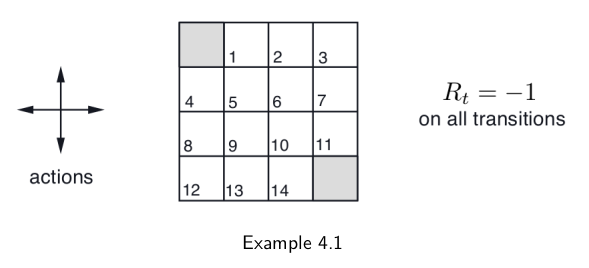
\includegraphics[width = 0.6 \textwidth]{example4.1.png}
\end{figure}

\end{exercise}

% -------------------------------------------------------------------------------- %

\begin{solution}

The action \textsc{down} taken from state 11 determinstically moves the agent
to the terminal state with reward -1, therefore

\begin{align*}
  q_\pi(11,\textsc{down}) = -1.
\end{align*}

\end{solution}

% -------------------------------------------------------------------------------- %
